\section{Protocole LIN}

\subsubsection*{Architecture}  
Le bus LIN est un système \textit{mono-maître et multi-esclaves}. Un seul maître initie toutes les communications, ce qui rend inutile toute fonction d'arbitrage. Le nombre d'esclaves n'est pas limité par la norme mais dépend des contraintes électriques. L'architecture est dite \textit{flexible}, car on peut ajouter des nœuds esclaves sans modifier les nœuds existants.  

\begin{figure}[H]
    \centering
    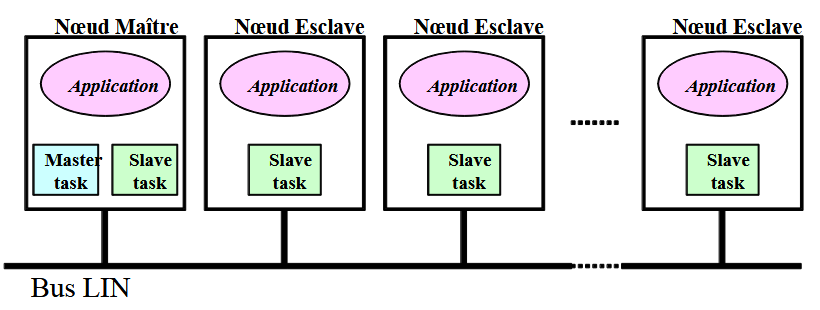
\includegraphics[width=0.8\linewidth]{images//Intro/Architecture_LIN_ME.png}
    \caption{Exemple d'architecture LIN}
    \label{fig:placeholder}
\end{figure}

\subsubsection*{Connexion}  
Le bus est constitué d'une \textit{seule ligne} reliée à chaque nœud par une sortie à collecteur ouvert. Le maître utilise une résistance de tirage de \SI{1}{k\ohm}, tandis que chaque esclave utilise \SI{30}{k\ohm}. La ligne est au niveau \textit{récessif (1)} lorsqu'aucun nœud ne force l'état, et au niveau \textit{dominant (0)} dès qu'au moins un nœud impose ce niveau.  

\begin{figure}[H]
    \centering
    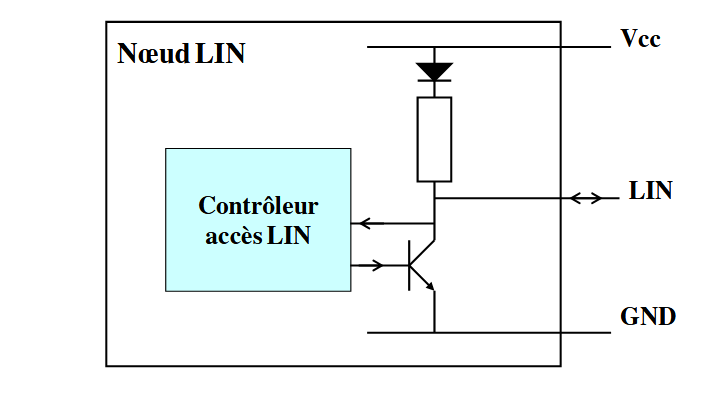
\includegraphics[width=0.5\linewidth]{images//Intro/Connection_LIN.png}
    \caption{Connexion physique d'un noeud à la ligne LIN}
    \label{fig:placeholder}
\end{figure}

\subsubsection*{Vitesse de transmission}  
Le débit varie de \SI{1}{kbit/s} à \SI{20}{kbit/s}, fixé pour une architecture donnée. Trois vitesses sont recommandées :  
\begin{itemize}
    \item \textbf{Lente} : 2400 bit/s,  
    \item \textbf{Moyenne} : 9600 bit/s,  
    \item \textbf{Rapide} : 19200 bit/s.  
\end{itemize}

\subsubsection*{Communications et trames}  
Les messages LIN sont composés de plusieurs champs :  
\begin{itemize}
    \item \textit{Synchronisation Break} : marque le début du message,  
    \item \textit{Synchronisation Field} : alignement des horloges (valeur 0x55),  
    \item \textit{Identification Field} : contenu et longueur des données, avec contrôle de parité,  
    \item \textit{Data Field} : octets d'information transmis du LSB vers le MSB,  
    \item \textit{Checksum Field} : somme de contrôle des données (modulo 256 inversée).  
\end{itemize}

\begin{figure}[H]
    \centering
    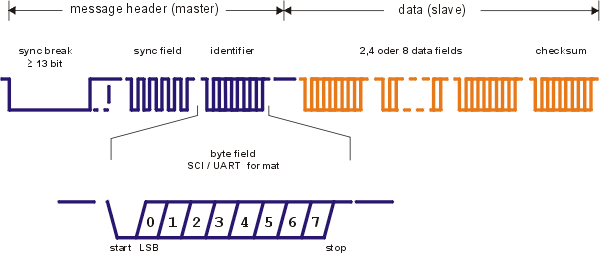
\includegraphics[width=0.8\linewidth]{images//Intro/Trame_LIN.png}
    \caption{Type de Trame Protocol LIN}
    \label{fig:placeholder}
\end{figure}

Une communication peut être de deux types :  
\begin{itemize}
    \item \textbf{Écriture} : le maître envoie l'intégralité du message,  
    \item \textbf{Lecture} : le maître envoie seulement l'entête, puis reçoit la réponse de l'esclave.  
\end{itemize}


